\documentclass[Persian]{cacna2023-fa}

%%%%%%%%%%%%%%%%%%%%%%%%%%%%%%%%%%%
\RequirePackage{xepersian}
\settextfont[BoldFont={YasBd.ttf},ItalicFont={YasIt.ttf},BoldItalicFont={YasBdIt.ttf}]{Yas.ttf}
\setdigitfont{Yas.ttf}
\usepackage{hyperref}


\setcounter{MaxMatrixCols}{20}


	
\begin{document}
		\begin{center}
		
\includegraphics[height=2.2cm, width=14.7cm]{header-fa}
	\end{center}
	\vspace*{0.5cm}
	
	
%%%%%%%%%%%%%%%%%%%%%%%%%%%%%%%%%%%%            شما از اینجا باید آغاز کنید:                  %%%%%%%%%%%%%%%%%%%%%%%%%%%                                                 
%%%%%%%%%%%%%%%%%%%%%%%%%%%%%%%%%%%%%%%%%%%%%%%%%%%%%%%%%%%%%%%%%%%%%%%%%%%%%%%%%%%%%%%%%%%%%%%%%%%%%%%%%%%%%%%%%%%%%%%%%%%
	\title{یافتن عدد وینر برای گراف پلی تیوفتن و ارائه یک چند جمله ای درجه سه با استفاده از عدد ${\rm PT_n}$}
	\maketitle
	
	\begin{center}
		
		
		\begin{alphafootnotes}
			ابوالفضل عقدائی $^{1}$%
			 ،	دکتر غلامحسین فتح تبار $^{2}$%
			
			$^{}$%
			\\[2mm]
			{\small
				$^{1}$دانشجوی کارشناسی  دانشکده علوم ریاضی، آمار و علوم کامپیوتر دانشگاه کاشان، کاشان، ایران
				
				\lr{\href{mailto:aghdaee80@std.kashanu.ac.ir}{aghdaee80@std.kashanu.ac.ir}}
			}
			\\[2mm]
			{\small
				$^{2}$دانشیار دانشکده علوم ریاضی، آمار و علوم کامپیوتر دانشگاه کاشان، کاشان، ایران
			
			
				\href{mailto:fathtabar@kashanu.ac.ir}{fathtabar@kashanu.ac.ir}
							}
		\\[2mm]
	
		\end{alphafootnotes}
			
	\end{center}

	
	
	\fancyhead[CO]{}
	\fancyhead[CE]{}

	

	%%%%%%%%%%%%%%%%%%%%%%%%

	%%%%%%%%%%%%% abstract %%%%%%%%%%%%%
	\hrulefill
	\begin{abstract}
		فرض کنید \lr{G =(V, E)} گراف مربوط به مولکول پلی تیوفن باشد،به طوری که مجمو رئوس با \lr{V} و مجموعه یال ها با E  نشان داده می شوند. مجموعه تمام فاصله های بین هر دو راس از گراف \lr{G} را پایای وینر گویند و با \lr{W(G)} نشان می دهند. دراین مقاله روشی برای بدست آوردن پایای گراف وینر و همچنین چند جمله ای درجه سه  برای گراف پلی تیوفن با استفاده از مقدار \lr{${\rm PT_n}$} که نمایانگر تعداد پنج ضلعی های موجود در گراف مورد نظر است ارائه شده است.
		\KeyWords{پلی تیوفن\/، پایای وینر، گراف }
		
	\end{abstract}
\hrulefill
	\section{مقدمه}
	زوج \lr{G = (V, E)} را که در آن V یک مجموعه ناتهی و E زیر مجموعه ای از تمام زیرمجموعه های دو عضوی 
	V است. که در این مقاله منظور از E اتم های موجود در مولکول پلی تیوفن و V  پیوندهای مولکولی بین اتم ها می باشد.

	پایای یک گراف عددی است که به گراف نسبت داده می شود طوری که نسبت به یکریختی
	گراف تغییر نمی کند. برای مثال تعداد یال های یک گراف پایای گراف است.

	تعداد یال های کوتاه ترین مسیر بین دو راس u و v از گراف G فاصله بین این دو راس گراف نامیده می شود و با 
	
	\lr{${\rm d_G}$ = (u, v)} نشان داده می شود.  
پایای وینر گراف G


\begin{equation}
	\mathcal{W}(G) =\sum_{\{ u,v\}  \subseteq V(G)}^{}\rm d_G(u, v)
\end{equation}

پایای وینر معرفی شده بانمادها و نام های متفاوت در علومی مانند علوم کامپیوتر،
مکانیک، مواد، شیمی داروسازی و ریاضی مورد استفاده قرار گرفته است.

آنچه مسلم است هارولد وینر اولین شیمی دانی است که مجموع فاصله های هر دو زوج 
رأس گراف را در درخت ها، برای تخمین نقطه ذوب آلکان ها درسال 1947، مورد توجه قرار داده است. وینر خودش از نام عدد مسیری برای این 
پایای گراف استفاده کرد و آن را با W 
نمایش داد. البته تعریف وینر اولین بار توسط شیمیدان ژاپنی به نام هارو هوسیا ارائه شد.
به نظر می رسد در نوشته های ریاضی مقدار وینر اولین بار درسال 1976 
مطالعه شده است. آن طور که شواهد نشان می دهد ریاضی دانان برای یک مدت زمان طولانی کاری که از
هارولد وینر در شیمی با استفاده از مجموع فواصل 
بین رئوس انجام داد، بی اطلاع بودند.\cite{1}



	 
	
	
	%%%%%%%%%%%%%%%%%%%%%%% NEXT SECTION	
	
	\section{پایای وینر}
	در این بخش، به معرفی و بررسی پایای وینر می پردازیم، فرض کنید
	G یک گراف باشد. پایای گراف G به صورت زیر تعریف می شود

	\begin{equation}
		\mathcal{W}(G) =\frac{1}{2} \sum_{u \in  V(G)} \sum_{v  \in V(G)}^{}\rm d_G(u, v)
	\end{equation}

	که درآن \lr{$\rm d_G(u, v)$} فاصله بین رأس u و v  است.
	اگر فاصله v از G  به صورت 

	
	\begin{equation}
		d(v, G)=\sum_{u  \in  V(G)}^{}\rm d(u, v)
	\end{equation}

	تعریف شود، آنگاه فرمول مربوط به پایای وینر را می توان بدین صورت 
	بازنویسی کرد:
	
	\begin{equation}
		\mathcal{W}(G) =\frac{1}{2} \sum_{v \in  V(G)} \rm d(v, G)
	\end{equation}


	


				\section{پایای وینر برای گراف پلی تیوفن}
				فرض کنید \lr{G =  ${\rm PT_n}$ }  که به جای 
				n هر مقداری می تواند قرار گیرد 
				که نشان دهنده تعداد پنج ضلعی های موجود در گراف
				پلی تیوفن می باشد.
				\begin{example}\label{ex1}
					برای مثال  ${\rm PT_1}$ برابر شکل زیر خواهد بود.
					
				\end{example}
				\begin{figure}[H]
					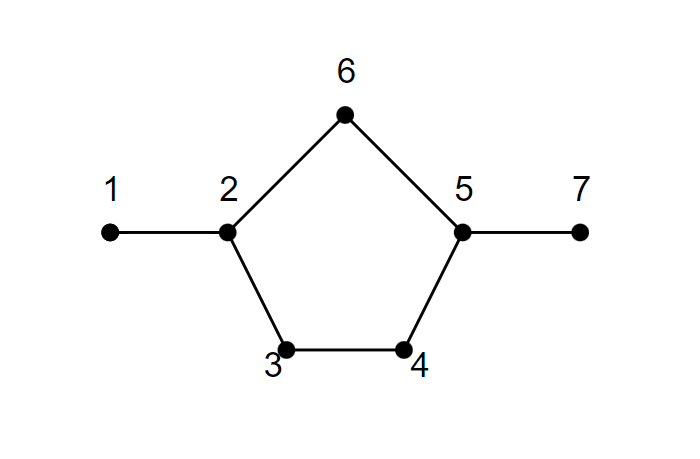
\includegraphics[width=7cm]{pt1.png}
					\caption{${\rm PT_1}$}
					\label{fig:pt1}
				  \end{figure}

				  حال هدف ما این هست که عددپایای وینر را برای گراف بالا بدست
				  بیاوریم. ابتدا ماتریسی 
				  مربعی که تعداد سطر و ستون آن برابر 7 می باشد را 
				  ایجاد کرده 
				  و در هر درایه فاصله دو نقطه 
				  ،متناظر را نوشته 
				  حال نتیجه ماتریس  به صورت زیر خواهد بود
				 

				  \[
\begin{array}{cc} 
&
\begin{array}{ccccccc} 
1 & 2 & 3 & 4 & 5 & 6 & 7
\end{array}
\\
\begin{array}{c}
1 \\
2 \\
3 \\
4 \\
5 \\
6 \\
7 \\
\end{array}
&
\left[
\begin{array}{ccccccc}
						0 & 1 & 2 & 3 & 3 & 2 & 4 \\
						1 & 0 & 1 & 2 & 2 & 1 & 3 \\
						2 & 1 & 0 & 1 & 2 & 2 & 3 \\
						3 & 2 & 1 & 0 & 1 & 2 & 2 \\
						3 & 2 & 2 & 1 & 0 & 1 & 1 \\
						2 & 1 & 2 & 2 & 1 & 0 & 2 \\
						4 & 3 & 3 & 2 & 1 & 2 & 0 \\
\end{array}
\right]
\end{array}
\]
				%   \begin{equation*}
				% 	\begin{bmatrix}{cccccccc}
				% 		0 & 1 & 2 & 3 & 3 & 2 & 4 \\
				% 		1 & 0 & 1 & 2 & 2 & 1 & 3 \\
				% 		2 & 1 & 0 & 1 & 2 & 2 & 3 \\
				% 		3 & 2 & 1 & 0 & 1 & 2 & 2 \\
				% 		3 & 2 & 2 & 1 & 0 & 1 & 1 \\
				% 		2 & 1 & 2 & 2 & 1 & 0 & 2 \\
				% 		4 & 3 & 3 & 2 & 1 & 2 & 0 \\
				% 	\end{bmatrix}
				% \end{equation*}


				فرض کنید درایه های ماتریس فوق را با ${\rm a_{ij}}$
				نشان دهیم پایای وینر برای ${\rm PT_1}$
			برابر فرمول زیر خواهد شد.
				\begin{equation}
					\mathcal{W}(\rm PT_1) = \frac{1}{2} \sum_{j=1}^{j=7}\sum_{i=1 }^{i=7}\rm a_{ij}
				\end{equation}
				\newline


				حال می خواهیم روشی مشترک برای بدست آوردن ${\rm PT_{2}}$ و بزرگ تر از آن 
				ارائه دهیم.
				\begin{definition}\label{def1}
					ماتریس زیر را ماتریس مکمل می نامیم که در پنج سطر و ستون پایانی 
				هر ماتریس نظیر جایگذاری می شود و درایه های آن ثابت است.
				\end{definition}
								\begin{equation*}
					\begin{bmatrix}
						0 & 1 & 2 & 2 & 3  \\
						1 & 0 & 1 & 2 & 2 \\
						2 & 1 & 0 & 1 & 1  \\
						2 & 2 & 1 & 0 & 2  \\
						3 & 2 & 1 & 2 & 0  \\
					
					\end{bmatrix}
				\end{equation*}
				\newline

				
				
				برای بدست آوردن ماتریس متناظر ${\rm PT_{2}}$ کافی ست مراحل زیر را طی کنیم .
				\newline
				\textbf{مرحله 1: }
				سطر و ستون ماتریس متناظر گراف ${\rm PT_{1}}$ را به تعداد 
				نقاط گراف ${\rm PT_{2}}$ گسترش می دهیم.


				تعداد نقاط از طریق فرمول بدست می آید.
				\begin{equation}
					 \rm PT_{n} \times  5 +2
				\end{equation}
				\newline
				\textbf{مرحله2: }
				به درایه های ستون آخر ماتریس ${\rm PT_{1}}$ به ترتیب 
				مقادیر
				یک، 
				دو، دو، یک و سه 
				را اضافه کرده  و در ستون های باقی مانده 
				جایگذاری می کنیم.
				\newline
				\textbf{مرحله3: }
				به درایه های سطر آخر ماتریس ${\rm PT_{1}}$ به ترتیب 
				مقادیر
				یک، 
				دو، دو، یک و سه 
				را اضافه کرده  و در سطرهای باقی مانده 
				جایگذاری می کنیم.
				\newline				
				\textbf{مرحله4: }
				حال ماتریس تشکیل شده شامل 12 سطر و ستون است که سطر و ستون های 
				8 تا 12 آن خالی هستند، 
				برای اینکه ماتریس مورد نظر ما کامل شود نیاز است که ماتریس
				مکمل را جایگذاری کنیم، با جایگذاری ماتریس مکمل ماتریس زیر 
				به وجود می‌آید. 
								 \begin{equation*}
									\rm PT_{2} =
					\begin{bmatrix}
						0 & 1 & 2 & 3 & 3 & 2 & 4 & 5 & 6 & 6 & 5 & 7 \\
						1 & 0 & 1 & 2 & 2 & 1 & 3 & 4 & 5 & 5 & 4 & 6 \\
						2 & 1 & 0 & 1 & 2 & 2 & 3 & 4 & 5 & 5 & 4 & 6 \\
						3 & 2 & 1 & 0 & 1 & 2 & 2 & 3 & 4 & 4 & 3 & 5 \\
						3 & 2 & 2 & 1 & 0 & 1 & 1 & 2 & 3 & 3 & 2 & 4 \\
						2 & 1 & 2 & 2 & 1 & 0 & 2 & 3 & 4 & 4 & 3 & 5 \\
						4 & 3 & 3 & 2 & 1 & 2 & 0 & 1 & 1 & 2 & 1 & 3 \\
						5 & 4 & 4 & 3 & 2 & 3 & 1 & 0 & 1 & 2 & 2 & 3 \\
						6 & 5 & 5 & 4 & 3 & 4 & 2 & 1 & 0 & 1 & 2 & 2 \\
						6 & 5 & 5 & 4 & 3 & 4 & 2 & 2 & 1 & 0 & 1 & 1 \\
						5 & 4 & 4 & 3 & 2 & 3 & 1 & 2 & 2 & 1 & 0 & 2 \\
						7 & 6 & 6 & 5 & 4 & 5 & 3 & 3 & 2 & 1 & 2 & 0 
					\end{bmatrix}
				\end{equation*}




				برای بدست آوردن ماتریس نظیر ${\rm PT_{n}}$ ما
				نیاز به ماتریس‌های نظیر ${\rm PT_{n-1}}$,${\rm PT_{n-2}}$...${\rm PT_{2}}$
				خواهیم داشت، که می‌توان با تکرار مراحل بالا به تعداد 
				\lr{n-1} بار 
				به ماتریس نظیر ${\rm PT_{n}}$ رسید.
				همچنین می‌توان از \href{https://github.com/abolfazlaghdaee/GraphTask/blob/main/wiener.py}{این برنامه}  برای محاسبه ماتریس نظیر و 
				پایای وینر استفاده کرد.


			







				



				\section{نتیجه‌گیری}\label{conc}
				برای دست‌یابی به عدد پایای وینر گراف پلی تیوفن با ${\rm PT_{n}}$های مختلف
				که تعداد پنج ضلعی‌های موجود در گراف را مشخص می‌کند می‌توان از 
				مراحلی که در بخش 3 بیان شد استفاده کرد و یا اینکه با 
				جایگذاری درفرمول زیر به آن رسید.
				\begin{equation}
					\mathcal{W}(X) = 12.5X^{3}+20X^{2}+7.5X+1
				\end{equation}




				
				\section*{تشکر و قدردانی}
				مراتب سپاس‌گزاری خود را از کمیته علمی برگزار کننده 
				کنفرانس و 
				همچنین جناب دکتر فتح تبار را اعلام
				می‌دارم. 
				روح پروفسور علی‌رضا اشرفی شاد و یادش گرامی باد.
				

			
				%%%%%%%%%%%%%%%%%%%%%%%%%%%%%%%%%%%%%%%%%%%
				\bibliographystyle{amsplain}
				\begin{thebibliography}{}

					\bibitem{1}
					\textbf{غ. فتح تبار، ا. محفوظ، مجموع فاصله‌های بین رئوس یک گراف، نشریه علمی ترویجی
				محاسبات نرم  5 (1395)،
				شماره دوم، 33-28}
					
				\end{thebibliography}
					
			\end{document}


